% July17, 1pm. What is written here is checked correct.
% but add example sections  

\documentclass[12pt]{article}

\setlength{\oddsidemargin}{-.5in} \setlength{\topmargin}{-.55in}
\setlength{\textwidth}{6.9in} \setlength{\textheight}{9.2in}

\usepackage{amsmath,amsthm,amssymb,amsopn,amsfonts}
\usepackage{graphics}
\usepackage{graphicx}

\newcommand{\onespace}{\renewcommand{\baselinestretch}{1}\normalsize}
\newcommand{\twospace}{\renewcommand{\baselinestretch}{1.3}\normalsize}
\newcommand{\Sobs}{{\mathcal{S}_{\mbox{\tiny{obs}}}}}
\newcommand{\R}{\mathbb{R}}
\newcommand{\mqed}{$\qed$ \medskip}

\newcommand{\Pry}{\mathbb{P}}
\newcommand{\Y}{{\mathcal Y}}
\newcommand{\UU}{{\mathcal U}}
\newcommand{\ve}{\textup{Vec}}
\newcommand{\Z}{\mathbb{Z}}
\newcommand{\tr}{\textup{trace}}


\newtheorem{theorem}{Theorem}
\newtheorem{proposition}[theorem]{Proposition}
\newtheorem{lemma}[theorem]{Lemma}
\newtheorem{corollary}[theorem]{Corollary}

\graphicspath{{./}{./../}{./../graphs/}{./graphs/}}
\twospace
\begin{document}

\title{A Fast Seeded Graph Matching Algorithm, and Seeded Matching of
Random Graphs from a Common Distribution}
\author{Donniell's writeup, in progress}

\maketitle
\begin{abstract} Given two graphs on the same number of vertices,
the graph matching problem is to find a bijection between the
two vertex sets which minimizes the number of adjacency disagreements
between the two graphs; this problem is NP-hard. The seeded graph
matching problem is the graph matching problem with an additional
constraint that the bijection assigns some particular vertices of
one vertex set to respective particular vertices of the other
vertex set. We modify the state-of-the-art approximate graph matching
algorithm of Vogelstein, Conroy, et al to make it an approximate
seeded graph matching algorithm.

Then we illustrate that two random graphs drawn from the same
distribution might be graph matched to each other in a way
that almost completely differs from the natural underlying
correspondence between the two graph's vertices within the
random graph model. However, seeding some of the vertices
according to this natural, underlying correspondence can
very significantly reduce---for the nonseeded vertices---
the difference between the seeded graph matching 
and the underlying correspondence. 
The effectiveness of the modified Vogelstein, Conroy et al 
approximate seeded graph matching algorithm in this context 
is illustrated with simulations, and through an example
of matching a library of linked Wikipedia documents in English to
the corresponding linked Wikipedia documents in French, an example
of matching an electrical network to its chemical counterpart in
a Caenorhabditis elegans (a particular roundworm) brain, and an example
of fraud detection by matching communication graphs from the failed
energy company Enron.
\end{abstract}

\newpage


\section{Setting and Overview}

All graphs in this manuscript are simple, ie the edges are undirected and
there are no loops or multiple edges. In other words, the adjacency matrices
for graphs are $\{ 0,1 \}$-valued square matrices that
are symmetric, with only zeros along the main diagonal.
This restriction to simple graphs is just a convenience; indeed,
all of our work and analysis can be naturally extended to settings
with more general graphs.

Suppose $G_1$ and $G_2$ are two graphs with respective vertex
sets $V_1$ and $V_2$ such that $\# V_1= \# V_2$. For any bijective function
$\phi : V_1 \rightarrow V_2$, the number of adjacency disagreements under $\phi$ is
defined to be
$ d(\phi):= \# \{ (u,v) \in V_1 \times V_1 :
[u \sim_{G_1} v  \mbox{ and } \phi(u) \not \sim_{G_2} \phi(v)] \mbox{ or }
[u \not \sim_{G_1} v  \mbox{ and } \phi(u) \sim_{G_2} \phi(v)]\}.$
The {\it graph matching problem} is to minimize $d(\phi)$ over all
bijective functions $\phi : V_1 \rightarrow V_2$.
This problem is NP-hard; in fact, even
the weaker problem of just deciding whether there exists a graph
isomorphism between $G_1$ and $G_2$ is notoriously of unknown complexity
(and, indeed, is suspected to belong to an intermediate complexity class
which is strictly between P and NP-complete). Thus, in particular, there are no
efficient algorithms known for graph matching, and it is not expected that
any exist.

Developing graph matching heuristics is a burgeoning field.
An excellent survey article by Conte, Foggia, Sansone, and Vento titled
``Thirty years of graph matching in pattern recognition"\cite{Thirty}
outlines successful application of approximate graph matching
to two-dimensional  and three-dimensional image analysis,
document processing, biometric identification, image databases,
video analysis, and biological and biomedical applications.
The current state-of-the-art algorithms can provide effective and realtime
approximate graph matching for graphs on $\approx 10^3$ vertices.\cite{VogCon}

In this manuscript, we will utilize the approximate graph matching
algorithm of Vogelstein, Conroy et al \cite{VogCon} which they
call ``FAQ" (an acronym for Fast Approximate Quadratic
Assignment Problem Algorithm); its running time is cubic in the number
of vertices and, in practice, the quality of the approximate solution and the
speed of the algorithm are state-of-the-art. The details of FAQ will
be specified later, in Section~\ref{mfaq}.
%(Very briefly, FAQ consists of casting the graph matching problem as
%maximizing a particular quadratic objective function subject to
%linear and integer constraints, then the integer constraints
%are relaxed to yield a quadratic program, then this quadratic
%program is solved by the Frank-Wolfe Method---in which the
%successive linear programs are cast as linear assignment problems and
%solved via the Hungarian Algorithm---and, finally, the output
%of Frank-Wolfe is projected so as to restore integrality.)


Suppose we are also given subsets $W_1 \subset V_1$, $W_2 \subset V_2$
such that $\# W_1= \# W_2$, and we are given a
fixed bijection $\psi: W_1 \rightarrow W_2$.
We define the {\it seeded graph matching problem} as the problem of
minimizing $d(\phi)$ over all bijections $\phi : V_1 \rightarrow V_2$
that agree with $\psi$ on $W_1$ (ie, for all $u \in W_1$, $\phi(u)=\psi(u)$).
The elements of $W_1$ are called {\it seeds} and the bijection
$\psi$ is a {\it seeding}. In Section~\ref{mfaq},
we modify the  approximate graph matching FAQ algorithm for 
use in approximate seeded graph matching.


When we say that ``$G_1$ on vertex set $V_1$, and $G_2$ on vertex set $V_2$
are random graphs independently drawn from the same distribution,
with {\it correspondence function}  $\Psi$ ",
(for the bijective function $ \Psi: V_1 \rightarrow V_2$),
we mean that there are specified probabilities for each of the
$2^{\# V_1 \choose 2}$ possible graphs on the vertex set $V_1$ and,
 from this probability distribution, the two graphs $G_1$ and $G_2$ are
independently realized and then---just in $G_2$---each vertex $u \in V_1$
is relabeled as $\Psi(u) \in V_2$, so that $G_1$ remains on vertex set
$V_1$ but $G_2$ now has vertex set $V_2$. The approximate graph matching
solution $\phi:V_1 \rightarrow V_2$ may be viewed as an approximation
for the underlying correspondence function $\Psi: V_1 \rightarrow V_2$, if
$\Psi$ is partially or completely unknown.

We will see in Section \ref{srg} that $\phi$ may be a very lousy
approximation for $\Psi$ in general, perhaps agreeing with $\Psi$ at
only a handful of vertices, not much different from chance.
%(Which is almost as bad as chance; the expected number
%of vertices where $\Psi$ agrees with a discrete-uniform randomly chosen
%bijection $V_1 \rightarrow V_2$ is $1$.)
However, we will also see that utilizing
some seeds $W_1 \subset V_1$---and the seeding function $\psi$
consisting of the restriction of $\Psi$ to $W_1$---can yield an approximate
seeded graph match solution which agrees with $\Psi$ on a much
more substantial fraction of the nonseeded vertices from $V_1$.

The structure of this paper is as follows:

In Section \ref{mfo} we
formulate the relaxation of the seeded graph matching problem.
In Section~\ref{straw} we describe a straight linear programming
approach---which we call ``SLP"---to approximately solve the
seeded graph matching problem. SLP is guaranteed to optimally solve
relaxed graph matching problems
(in contrast to all current state-of-the-art algorithms), and
SLP runs in polynomial time. Thus, assuming that we give
up on the intractable unrelaxed (integral) seeded graph matching
problem in favor of solving a relaxation and projecting it to the nearest
integer solution, then it can be argued that SLP is the best
choice for this {\it if we don't care at all about running time
except to demand that running time be polynomial}.
Thus, SLP will serve as
an excellent ``straw man" here, a benchmark to compare other
algorithms against to assess quality of solution (even though SLP is
many orders of magnitude slower than state-of-the-art).

In Section \ref{mfaq} we adapt the FAQ algorithm of
Vogelstein, Conroy et al into an algorithm for approximate
seeded graph matching; in Section \ref{srg} we observe that
modified FAQ seems to be just as effective as SLP (while running
many orders of magnitude faster). We see that for random graphs
drawn from the same distribution, the approximate graph matching
will not in general agree much with the underlying correspondence
function, but seeding can dramatically improve such agreement
for the nonseeded vertices. Examples that illustrate this
are (Section \ref{wiki}) matching a library of linked Wikipedia
documents in English to the corresponding linked Wikipedia documents
in French, (Section \ref{celegans}) an example
of matching an electrical network to its chemical counterpart in
a Caenorhabditis elegans brain, and (Section \ref{enron}) an example
of fraud detection by matching communications networks from the failed
energy company Enron.

\newpage

\section{The relaxed seeded graph matching problem \label{mfo}}

We are interested in solving the seeded graph matching problem but, as
discussed earlier, the seeded graph matching problem is NP-hard,
and we thus have no expectation that there even exists an efficient
algorithm. So we seek approximate solutions that can be
efficiently computed.

In this section we express the seeded graph matching
problem as an optimization problem with integer constraints, and then
we relax the integer constraints by replacing them with nonnegativity
constraints. Of course, when solving a relaxation, the solution
may not in general be integer valued, and as such it would not even
be appropriate as an approximate solution to the unrelaxed original
problem. However, we will then project the solution of the relaxed
optimization problem to the nearest member of the feasible
region of the unrelaxed problem, and we then declare that to be the
approximate solution of the original (unrelaxed) problem.


Recall that $G_1$ is a graph on vertex set $V_1$, $G_2$ is a
graph on vertex set $V_2$ such that $\#V_1=\#V_2$, the set of seeds
$W_1$ is a subset of $V_1$, $W_2$ is a subset of $V_2$ such that
$\#W_1=\#W_2$, and bijection $\psi:W_1 \rightarrow W_2$
is the seeding. Without loss of generality, we will take
$V_1$ and $V_2$ to each be the set of integers $\{1,2,\ldots,m+n\}$,
we will take $W_1$ and $W_2$ to each be the set of integers
$\{ 1,2,\ldots,m \}$, we will take $\psi$ to be the identity
function, for some fixed nonnegative integer $m$ and positive integer $n$.
Let $A,B \in \R^{(m+n)\times (m+n)}$ be the adjacency matrices
for $G_1$ and $G_2$, respectively; this means that
for all $i,j \in \{1,2,\ldots,m+n\}$
it holds that $a_{ij}=1$ or $0$ according as $i \sim_{G_1} j$ or not,
and  $b_{ij}=1$ or $0$ according as $i \sim_{G_2} j$ or not.
It will soon be useful to let $A$ and $B$ be partitioned as
\[  A =\left [
\begin{array}{cc} A_{11} & A_{12} \\ A_{21} & A_{22} \end{array} \right ]
\ \ \ \ \ \ \ \ \ B =\left [
\begin{array}{cc} B_{11} & B_{12} \\ B_{21} & B_{22} \end{array} \right ]
\]
where $A_{11},B_{11}\in \R^{m \times m}$,
$A_{12},B_{12}\in \R^{m \times n}$, $A_{21},B_{21}\in \R^{n \times m}$, and
$A_{22},B_{22}\in \R^{n \times n}$.


It is clear that  the seeded graphmatch problem is to
minimize $\|A-(I_{m \times m}\oplus P)B(I_{m \times m}\oplus P)^T\|_1$ over all $n \times n$ permutation matrices $P$, where $I_{m \times m}$ is the $m$-by-$m$
identity matrix, $\oplus$ is the direct sum of matrices,
and $\| \cdot \|_1$ is the $\ell_1$  vector norm on matrices;
say the optimal $P$ is $\tilde{P}$.
Then the corresponding bijection $\phi_{\tilde{P}}: \{1,2,\ldots,m+n\} \rightarrow \{1,2,\ldots,m+n\}$
defined as, for all $i \in \{1,2,\ldots,m\}$, $\phi_{\tilde{P}}(i)=i$ and,
for all $i,j \in \{1,2,\ldots,n\}$, $\phi_{\tilde{P}} (i+m)=j+m$ precisely when $\tilde{p}_{ij}=1$, is the bijection which solves the seeded graphmatch problem.

Of course, this optimization problem is equivalent to minimizing
$\|A(I_{m \times m}\oplus P)-(I_{m \times m}\oplus P)B\|_1$ or
$\|A-(I_{m \times m}\oplus P)B(I_{m \times m}\oplus P)^T\|_2$ or
$\|A(I_{m \times m}\oplus P)-(I_{m \times m}\oplus P)B\|_2$, over all
permutation matrices $P$,
where $\| \cdot \|_2$ is the $\ell_2$ vector norm on matrices.
Expanding out $\|A-(I_{m \times m}\oplus P)B(I_{m \times m}\oplus P)^T\|_2^2=
\|A\|_2^2 + \|B\|_2^2
- 2 \cdot \tr A^T(I_{m \times m}\oplus P)B(I_{m \times m}\oplus P^T)$,
we see that this optimization problem is equivalent to maximizing $\tr A^T(I_{m \times m}\oplus P)B(I_{m \times m}\oplus P^T)$
over permutation matrices $P$.\footnote{Note that although $A$ and $B$ are
symmetric matrices, we nonetheless keep transposes in place wherever
they are present to enable further generalization;
our analysis will not change if we instead were
in a broader setting where $A$ and $B$ are
generic (nonsymmetric, nonhollow, and/or nonintegral) matrices in
$\R^{(m+n)\times (m+n)}$.}

Although we don't expect to ever find an efficient
algorithm for seeded graph matching, we will next have efficient
algorithms for solving a relaxation of seeded graph matching.
In Section \ref{straw}, where we define the algorithm SLP,
we will minimize $\|A(I_{m \times m}\oplus P)-(I_{m \times m}\oplus P)B\|_1$
subject to the constraint that $P$ is a doubly stochastic matrix,
which means that $P \in \R^n$ such that $P \vec{1}_n=\vec{1}_n$, $P^T \vec{1}_n=\vec{1}_n$, and $P \geq 0_{n \times n}$ coordinatewise,
where $0_{n \times n}$ is the $n$-by-$n$ matrix of zeros and $\vec{1}_n$ is the $n$-vector of all ones. In Section \ref{mfaq}, where we define the
modified FAQ algorithm,  we maximize
$\tr A^T(I_{m \times m}\oplus P)B(I_{m \times m}\oplus P^T)$
over all doubly stochastic matrices $P$.
Indeed, both of these are relaxations of the seeded graphmatch
problem in the sense that
if we were to add integrality constraints---that $P$ is
integer-valued---then we would precisely return to the constraint
that $P$ is a permutation matrix, hence we would have
returned to the seeded graphmatch problem.


There is one last detail to cover in this section.
We will indeed efficiently solve these relaxations
of the seeded graph matching problem, say the
solution is the doubly stochastic matrix $\tilde{P}$; but, if
$\tilde{P}$ is not a permutation matrix, then how do we get
out of $\tilde{P}$ a meaningful approximate solution to the seeded
graph matching problem? The answer is that we will do one more step;
we will find the permutation matrix $\tilde{Q}$ which solves the
optimization problem min $\| Q - \tilde{P} \|_1$ subject to $Q$ being
a permutation matrix, and finally $\phi_{\tilde{Q}}$ is our approximate
seeded graphmatch solution. To solve this latter
optimization problem, observe that for any permutation matrix $Q$
\begin{eqnarray*}
\|Q - \tilde{P}\|_1 & = & \sum_{i,j \in \{1,2,\ldots,n \}:q_{ij}\ne 1}\tilde{p}_{ij}
+ \sum_{i,j \in \{1,2,\ldots,n \}:q_{ij}=1}(1-\tilde{p}_{ij}) \\  & = &
\sum_{i,j \in \{1,2,\ldots,n \}}\tilde{p}_{ij} +
 \sum_{i,j \in \{1,2,\ldots,n \}:q_{ij}=1}(1-2\tilde{p}_{ij}) \\
 & = & n+ n -2 \cdot \sum_{i,j \in \{1,2,\ldots,n \}:q_{ij}=1}\tilde{p}_{ij}\\
 & = & 2n -2 \ \tr Q^T \tilde{P} .
 \end{eqnarray*}
 Thus,  minimizing $\| Q - \tilde{P} \|_1$ subject to $Q$ being a permutation
matrix is equivalent to maximizing $\tr Q^T \tilde{P}$ subject to $Q$ being
a permutation matrix; this latter optimization formulation is precisely
a formulation of the well-known linear assignment problem, and it
is efficiently solvable in $O(n^3)$ time with Edmonds and Karp's [cite]
and Tomizawa's [cite] implementation
of the so-called Hungarian Algorithm.
In this manner we can efficiently obtain
$\phi_{\tilde{Q}}$, which is our approximate seeded graphmatch solution.



\section{SLP algorithm: the straw man \label{straw}}

This section describes the straight linear programming ``SLP" approach for
approximate seeded graph matching. In SLP, we first optimally
solve the relaxed seeded graph matching problem: minimize
$\|A(I_{m \times m}\oplus P)-(I_{m \times m}\oplus P)B\|_1$
subject to the constraint that $P$ is a doubly stochastic matrix. This is
done by solving the linear programming problem described below
with an interior point method. Then SLP projects the linear program's
solution to the nearest permutation matrix and converts that
permutation matrix to a seeded graph matching $\phi$ in the manner
described at the end of Section \ref{mfo}. This $\phi$ is the output of SLP.
(Straight linear programming has historically been used to tackle (nonseeded)
graph matching in general, see eg \cite{sixteen}.)

SLP runs in polynomial time since it just involves solving one linear
programming problem with an interior point method and then one use of the Hungarian
Algorithm to project the linear pragram's
solution to a permutation matrix. However, solving this linear program
directly is relatively expensive, and therefore the running time of SLP
is not even remotely as fast as the modified FAQ algorithm
described in Section \ref{mfaq}. However, SLP is guaranteed to
optimally solve the  relaxed seeded graph matching problem in
polynomial time (as opposed to all of the other state-of-the-art
algorithms, which may not converge or may converge to stationary points
or local minima that are not globally optimal) and, for this reason,
we use SLP as the ``straw man" to compare the quality of the
output of the modified FAQ algorithm against the quality
of the output of SLP. Indeed, if we did not care about running
time except that it be polynomial, then an argument can be made that
SLP is the right algorithm to use for approximate seeded graph matching.


We now spell out the linear program that expresses
minimize $\|A(I_{m \times m}\oplus P)-(I_{m \times m}\oplus P)B\|_1$
subject to the constraint that $P$ is a doubly stochastic matrix. Note that
\begin{eqnarray*}  \| A(I_{m \times m}\oplus P)-(I_{m \times m}\oplus P)B\|_1
&=& \left \|
\left [
\begin{array}{cc} A_{11} & A_{12}P \\ A_{21} & A_{22}P \end{array}
\right ]
-
\left [
\begin{array}{cc} B_{11} & B_{12} \\ PB_{21} & PB_{22} \end{array}
\right ] \right \|_1 \\
&=& \|A_{11}-B_{11}\|_1 + \| \left ( I_{n \times n} \otimes A_{22}
 -B^T_{22} \otimes I_{n \times n} \right ) \ve P \|_1
\\ & &   + \| \left ( ( I_{n \times n} \otimes  A_{12} ) \ve P \right )
- \ve B_{12} \|_1
+ \| \left (  ( B^T_{21} \otimes I_{n \times n} ) \ve P \right ) - \ve A_{21} \|_1
\end{eqnarray*}
where $\otimes$ denotes the Kronecker product of two matrices, and ``$\ve$"
of a matrix denotes the concatenation the columns of the argument matrix into a single,
long column. By introducing two sets of slack variables $\epsilon^+$ and $\epsilon^-$
to capture $\ell_1$ discrepancy, and by noting that the conditions $P \vec{1}_n=\vec{1}_n$
and $P^T \vec{1}_n=\vec{1}_n$ can be expressed as
$(I_{n \times n}  \otimes \vec{1}^T_{n}) \ve P = \vec{1}_n$ and
$(\vec{1}^T_{n} \otimes I_{n \times n}) \ve P = \vec{1}_n$, we thus obtain
relaxed seeded graphmatch as the following linear program in standard form:


\[ \min
\left [ \begin{array}{c} \vec{0}_{n^2} \\ \vec{1}_{n^2+2mn} \\ \vec{1}_{n^2+2mn} \end{array}
\right ] ^T
\left [ \begin{array}{c} \textup{vec}P \\ \epsilon^+ \\ \epsilon^- \end{array}
\right ] \ \ \ \ \ \ \ \ \ \ \ \ \ \ \ \ \ \ \ \ \ \ \ \ \ \ \ \ \ \ \ \ \ \
 \ \ \ \ \ \ \ \ \ \ \ \ \ \ \ \ \ \ \ \ \ \ \ \ \ \ \ \ \ \ \ \ \ \ \ \ \ \ \
 \ \ \ \ \ \ \ \ \ \ \ \ \ \ \ \ \ \ \
\]
\[ \mbox{such that }
\left [ \begin{array}{c} I_{n \times n} \otimes A_{22}
 -B^T_{22} \otimes I_{n \times n}
  \\ I_{n \times n} \otimes  A_{12}
  \\ B^T_{21} \otimes I_{n \times n}
  \\ I_{n \times n}  \otimes \vec{1}^T_{n}
  \\ \vec{1}^T_{n} \otimes I_{n \times n}
   \end{array}
 \begin{array}{|cc}  & \\  I_{(n^2 + 2mn)\times (n^2+2mn)} &
 -I_{(n^2+2mn) \times (n^2+2mn)} \\ &  \\ 0_{2n \times (n^2+2mn)} & 0_{2n\times (n^2+2mn)}
 \end{array}
   \right ]
\left [ \begin{array}{c} \textup{vec}P \\ \epsilon^+ \\ \epsilon^- \end{array}
\right ]
=
\left [ \begin{array}{c}  \vec{0}_{n^2} \\ \textup{vec}B_{12} \\
\textup{vec}A_{21}\\ \vec{1}_n \\ \vec{1}_n  \end{array} \right ]
\]
\[ \mbox{and } \left [ \begin{array}{c} \textup{vec}P \\ \epsilon^+ \\ \epsilon^- \end{array}
\right ] \geq \vec{0}_{3n^2+4mn} \ \ \ \ \ \ \ \
\ \ \ \ \ \ \ \ \ \ \
\mbox{where } \mbox{vec}P \in \R^{n^2}
\ \ \mbox{and} \ \
\epsilon^+,\epsilon^- \in \R^{n^2+2mn} .
 \ \ \ \ \
\ \ \ \ \ \ \ \ \ \ \ \ \ \ \ \ \ \ \ \ \ \ \ \ \ \ \ \ \ \
\ \ \ \ \ \ \ \ \ \ \ \ \ \ \ \ \ \
\]

This linear program can be efficiently solved by an interior point method. This
concludes the description of SLP.



\section{Modified-FAQ for seeded graph matching \label{mfaq}}

In this section we modify the state-of-the-art approximate graph matching
algorithm of Vogelstein, Conroy, et al, which they call FAQ, so that it can
be used for approximate seeded graph matching. As mentioned before, the
seeded graph matching problem
can be expressed as that of maximizing
$\tr A^T(I_{m \times m}\oplus P)B(I_{m \times m}\oplus P^T)$
over all permutation matrices $P$ and, as mentioned before,
we don't expect that there is an efficient algorithm for this,
so we instead consider the relaxation,
which is maximizing $\tr A^T(I_{m \times m}\oplus P)B(I_{m \times m}\oplus P^T)$
over all doubly stochastic matrices $P$.
When a solution (or approximate solution) to the relaxed problem is found,
then it is projected to the nearest permutation matrix and converted 
to a seeded graph matching $\phi$
in the manner described at the end of Section \ref{mfo}.
 This $\phi$ is the output of modified-FAQ.


The modified FAQ algorithm solves (or approximately
solves) the relaxed seeded graph matching problem---maximize
$\tr A^T(I_{m \times m}\oplus P)B(I_{m \times m}\oplus P^T)$
subject to $P$ being a doubly stochastic matrix---by using the
Frank-Wolfe Method, which is an iterative procedure that
involves successively solving linearizations. It turns out that the
linearizations can be cast as linear assignment problems
that are solved with the Hungarian Algorithm. So, although SLP
involves solving only one linear program and here we will solve
a succession of linear programs, nonetheless the special form of
the linear programs in this section allows for the Hungarian Algorithm
to be employed, which is orders of magnitude faster than  an
interior point method for solving a linear program.

We first briefly review the Frank-Wolfe Method before proceeding
to apply it. The general kind of
 optimization problem for which the Frank-Wolfe Method is used is
  \begin{eqnarray} \label{i} \textup{(FWP)  \ \ \ Minimize}
\ \ \  f(x) \ \textup{   such that   } \
x \in S,
\end{eqnarray}
where $S$ is a polyhedral set (ie is described by linear
constraints) in a Euclidean space of some dimension,
and the function $f:S \rightarrow \R$ is continuously differentiable.
A starting point $x^{(1)} \in S$ is chosen in some fashion,
perhaps arbitrarily. For $i=1,2,3,\ldots$, the following is done.
The function $\tilde{f}^{(i)}:S \rightarrow \R$ is defined to be the
first order (ie linear) approximation to $f$ at $x^{(i)}$---that is,
$\tilde{f}^{(i)}(x):=f(x^{(i)})+\nabla f(x^{(i)})^T(x-x^{(i)})$;
then solve the linear program: minimize $\tilde{f}^{(i)}(x)$ such that $x \in S$
(this can be done efficiently since it is a linear
objective function with linear constraints, and note that, by ignoring additive constants, the objective function of this subproblem can be
abbreviated: minimize $\nabla f(x^{(i)})^Tx$
such that $x \in S$), say the solution is
$\tilde{x}^{(i)} \in S$. Now, the point $x^{(i+1)} \in S$ is defined
as the solution to: minimize $f(x)$ such that $x$ is on the line segment
from $x^{(i)}$ to $\tilde{x}^{(i)}$ in $S$. (This is a just a one dimensional
optimization problem; in the case where $f$ is quadratic this can
be exactly solved analytically.) Go to the next $i$,
and terminated this iterative procedure
when the sequence of iterates $x^{(1)}$, $x^{(2)}$, $x^{(3)}$, \ldots stops
changing much or develops a gradient close enough to zero. This
concludes our review of the Frank-Wolfe Method.

We now describe how modified FAQ employs the Frank-Wolfe Method to
solve the relaxed  seeded graph matching problem.
The objective function here is
\begin{eqnarray*}  f(P)  & =  &   \tr \left (
\left [  \begin{array}{cc}  A^T_{11} & A^T_{21} \\ A^T_{12} & A^T_{22}  \end{array} \right ]
\left [  \begin{array}{cc}  I_{m \times m} & 0_{m \times n}
\\ 0_{n \times m} & P  \end{array} \right ]
\left [  \begin{array}{cc}  B_{11} & B_{12} \\ B_{21} & B_{22}  \end{array} \right ]
\left [  \begin{array}{cc}  I_{m \times m} & 0_{m \times n}
\\ 0_{n \times m} & P^T  \end{array} \right ]
\right ) \\
& = & \tr \left (
\left [  \begin{array}{cc}  A^T_{11} & A^T_{21} \\ A^T_{12} & A^T_{22}  \end{array} \right ]
\left [  \begin{array}{cc}  B_{11} & B_{12}P^T \\ PB_{21} & PB_{22}P^T  \end{array} \right ]
\right )\\
& = & \tr A_{11}^TB_{11}+ \tr A_{21}^TPB_{21}+\tr A_{12}^TB_{12}P^T
+ \tr A_{22}^TPB_{22}P^T \\
& = &  \tr A_{11}^TB_{11}+ \tr P^T A_{21}B_{21}^T+\tr P^TA_{12}^TB_{12}
+ \tr A_{22}^TPB_{22}P^T
\end{eqnarray*}
which has gradient
\begin{eqnarray*}
\nabla (P):=A_{21}B_{21}^T+A_{12}^TB_{12}+A_{22}PB_{22}^T+A_{22}^TPB_{22} .
\end{eqnarray*}

We start the Frank-Wolfe Algorithm at the doubly stochastic matrix
$\tilde{P}=\frac{1}{n}\vec{1}_n \vec{1}_n^T$. (This is only for
simplicity, and any other choice of doubly stochastic $\tilde{P}$ might
be as effective). In the next paragraph we describe a single step in the
Frank-Wolfe algorithm. Such steps are repeated iteratively until
the iterates empirically converge.


Given any particular doubly stochastic matrix $\tilde{P} \in \R^{n \times n}$
the Frank-Wolfe-step linearization involves maximizing $\tr Q^T \nabla(\tilde{P})$ over all of the doubly stochastic matrices $Q \in \R ^{n \times n}$.
This is precisely the linear assignment problem (since it is not hard to show that
the optimal doubly stochastic $Q$ can in fact be selected to be
a permutation matrix) and so
the Hungarian Algorithm
will in fact find the optimal $Q$, call it
$\tilde{Q}$.
The next task in the Frank-Wolfe algorithm step
will be maximizing the objective function over the line
segment from $\tilde{P}$ to $\tilde{Q}$;  ie maximizing $g(\alpha):=f(\alpha \tilde{P}
+(1-\alpha ) \tilde{Q})$ over $\alpha \in [0,1]$. Denote
$c:=\tr A^T_{22} \tilde{P} B_{22} \tilde{P}^T$ and
$d:=\tr (A^T_{22} \tilde{P} B_{22} \tilde{Q}^T +
    A^T_{22} \tilde{Q} B_{22} \tilde{P}^T)$ and
$e:=\tr A^T_{22} \tilde{Q} B_{22} \tilde{Q}^T$ and
$u:=\tr ( \tilde{P}^TA_{21}B_{21}^T   + \tilde{P}^TA_{12}^TB_{12} )$ and
$v:=\tr ( \tilde{Q}^TA_{21}B_{21}^T   + \tilde{Q}^TA_{12}^TB_{12} )$. Then
(ignoring the additive constant $\tr A_{11}^TB_{11}$ without loss of
generality, since it won't affect the maximization)
we have $g(\alpha)=c \alpha^2+d \alpha (1-\alpha)
+e(1-\alpha)^2+u \alpha + v(1-\alpha)$  which simplifies to
$g(\alpha)=(c-d+e)\alpha^2+(d-2e+u-v)\alpha + (e+v)$. Setting the
derivative of $g$ to zero yields potential critical point
$\tilde{\alpha}:=\frac{-(d-2e+u-v)}{2(c-d+e)}$ (if indeed
$0 \leq \tilde{\alpha}\leq 1$); thus the next Frank-Wolfe algorithm
iterate will either be $\tilde{P}$ (in which case algorithm would halt)
or $\tilde{Q}$ or $\tilde{\alpha}\tilde{P}+(1-\tilde{\alpha})\tilde{Q}$, and
the objective functions can be compared to decide which of these three matrices
will be the $\tilde{P}$ of the next Frank-Wolfe step.

At the termination of the Frank-Wolfe Algorithm, we have a solution, or
an approximate solution, to the relaxed
seeded graph matching problem. This concludes the description of the
modified FAQ algorithm. By limiting the number of Frank-Wolfe steps to 
a constant, the running time is cubic in the number of vertices, since that 
is the complexity of the Hungarian Algorithm. There is no appreciable 
difference in running time between modified FAQ and FAQ, and we
thus have state-of-the-art running time, in practice.


\section{Seeding of random graphs  \label{srg}}

In this section, we illustrate that for random graphs
drawn from the same distribution, the approximate graph matching
may not in general agree much with the underlying correspondence
function, but seeding might dramatically improve such agreement
for the nonseeded vertices.

\subsection{Bernoulli random graphs}

If a matrix
$\Omega \in [0,1]^{k \times k}$, for some positive
integer $k$, is symmetric with zeros along the
main diagonal then  a {\it Bernoulli}($\Omega$) random
graph is a random graph on the vertices $\{1,2,\ldots,k\}$
wherein, for all $i,j$ such that $i<j$, the probability that
$i \sim j$ is $\Omega_{ij}$, independently for all such pairs $i,j$.

Given such a matrix of parameters
$\Omega \in [0,1]^{k \times k}$ and a positive
integer $n$ less than $k$, consider the following experiment,
which we will call Experiment$(\Omega,n)$:
Independently realize two Bernoulli($\Omega$) random graphs.
Call the first graph $G_1$.
Call the second graph $G_2$, but only after permuting/relabeling its vertices
with an arbitrarily selected bijective correspondence function $\Psi:
\{1,2,\ldots,k \} \rightarrow \{ 1,2,\ldots,k \}$, where $\Psi$ is
arbitrary except that for all $i=1,2,\ldots,k-n$ it holds that
$\Psi(i)=i$. Then, for each of $m=0,1,2,\ldots,k-n$, compute the modified-FAQ seeded
graph matching $\phi^{(m)}$ between the subgraphs~of~$G_1$~and~$G_2$~induced by the
$m+n$ vertices $V_1^{(m)}=V_2^{(m)}:=\{k-n-m+1,k-n-m+2,k-n-m+3,\ldots, \ \ k\}$,
 using the seeding $\Psi$ on the $m$ seed vertices
 $W_1^{(m)}=W_2^{(m)}:=\{k-n-m+1,k-n-m+2,k-n-m+3,\ldots,\ \ k-n\}$
(and there are $n$ nonseeded vertices $\{ k-n+1,k-n+2,k-n+3, \ldots, \ \ k \}$).
The {\it match ratio} $\delta^{(m)}:=\frac{\# \{ v \in V_1^{(m)} \backslash W_1^{(m)}: \phi^{(m)}(v)=\Psi (v)\}}{n} $ is the fraction of the $n$ nonseeded vertices where $\phi^{(m)}$ agrees with correspondence function~$\Psi$. Note that
there are always the same $n$ nonseeded vertices that we
are interested in matching across the two graphs
and, as $m=0,1,2,\ldots$, each increment of $m$ adds
to the utilized instance a new seed vertex, which is seeded to agree with
the assignment function~$\Psi$. When $m=0$ the graph matching
problem instance isn't seeded at all.

In Figure~XXa, we plotted the match ratio $\delta^{(m)}$ against
$m=0,1,2,\ldots,90$, averaged over $65$ repetitions of  Experiment$(\Omega,30)$, where
$k=120$ and each of the lower triangular elements of each of the $65$ parameter
matrices $\Omega$ was independent, Uniformly distributed on
the interval $(0,1)$. In Figure~XXb, we did the same as was done to get
Figure~XXa, except that we used SLP instead of modified-FAQ to do the
seeded graph matching. Several observations should be made:

Note that if instead of graph matching we just discrete-uniform-randomly
selected any bijection between the unseeded vertices of the two graphs,
the expected number of agreements between such a random bijection and
the assignment function is exactly $1$. Thus, here
``chance" would have match ratio $\frac{1}{30}=.0333$, which is not that
much different than the match ratio $\delta^{(0)} \approx .05$
when there were no seeds. As seeds are added here, there was a dramatic
increase in the match ratio. When there were
around $30$ seeds then the match ratio here was more than
$.50$, and where there were around $60$ seeds then the
match ratio here was more than $.90$, and there empirically seems
to be a close-to-linear relationship between  $\delta^{(m)}$ and $m$,
for $m$ between $0$ and $60$.\\

ADD BRIEF EXPLANATION AS TO WHY THIS IS SURPRISING/ NOT SURPRISING\\


Also note that, unlike SLP, modified-FAQ is not
guaranteed to optimally solve the relaxed seeded graph matching problem
but, nonetheless, the empirical performance here of modified-FAQ was
not that different than the empirical performance of SLP. However,  
on a personal computer, the computing time to perform the experiments for
Figure XXb with SLP was around $80$ hours, whereas the computing time
to perform the experiments for Figure XXa with modified-FAQ was
only $134$ seconds.

\newpage

\subsection{Two-class random graphs}


Suppose that we are given a positive integer $k$,
a function $\gamma: \{ 1,2,\ldots,k \} \rightarrow
\{0,1\}$, and also $p,q,r$ in the real interval $[0,1]$.
A Two-Class$(\gamma,p,q,r)$ random graph is a random
graph on the vertices $\{1,2,\ldots,k\}$ wherein, for
all $i,j$ such that $i<j$, the probability that $i \sim j$
is $p$, $q$, or $r$, according as $\gamma(i)=\gamma(j)=0$, or
$\gamma(i)=\gamma(j)=1$, or $\gamma(i)\ne \gamma(j)$, independently for
all such pairs $i,j$. The vertices in
$\{i:1 \leq i \leq k, \gamma(i)=0 \}$ will be called the {\it first class}
of vertices, and the vertices in $\{i:1 \leq i \leq k, \gamma(i)=1 \}$
will be called the {\it second class} of vertices. The graph
might represent, for instance, a social network, with the first class consisting
of innocent people and the second class consisting of scheming fraudsters,
where the probability of two vertices/people communicating
just depends on whether they are both nonfraudsters, or both frausters,
or exactly one of them is a fraudster. (In Section \ref{enron} we will
deal with an actual social network of email messages/ edges
among Enron employees/ vertices, where some of the employees are innocent
and some of them were scheming to commit fraud.)


Given such two-class-random-graph parameters
$\gamma,p,q,r$  and given a positive
integer $n$ less than~$k$, consider the following experiment,
which we call Experiment$(\gamma,p,q,r,n)$:
Independently realize two
Two-Class$(\gamma,p,q,r)$ random graphs. Call the first graph $G_1$.
Call the second graph $G_2$, but only after permuting/relabeling its vertices
with an arbitrarily selected bijective correspondence function $\Psi:
\{1,2,\ldots,k \} \rightarrow \{ 1,2,\ldots,k \}$;
$\Psi$ is arbitrary except that for
all $i=1,2,\ldots,k-n$ it holds that $\Psi(i)=i$. Then, for each of
$m=0,1,2,\ldots,k-n$, compute the modified-FAQ seeded
graph matching $\phi^{(m)}$ between the subgraphs of $G_1$ and $G_2$ induced by the
$m+n$ vertices $V_1^{(m)}=V_2^{(m)}:=\{k-n-m+1,k-n-m+2,k-n-m+3,\ldots, \ \ k\}$,
 using the seeding $\Psi$ on the $m$ seed vertices
 $W_1^{(m)}=W_2^{(m)}:=\{k-n-m+1,k-n-m+2,k-n-m+3,\ldots,\ \ k-n\}$
(and there are $n$ nonseeded vertices $\{ k-n+1,k-n+2,k-n+3, \ldots, \ \ k \}$).
Of course, all first class vertices are stochastically
indistinguishable one from another, and all second class vertices
are stochastically indistinguishable one from another. Thus, our goal
ought not be to have $\phi^{(m)}$ agree with the correspondence function
$\Psi$ but, rather, our goal is that they agree about the class of
as many vertices as possible. With this in mind, we define the match ratio
to be $\delta^{(m)}:=\frac{\# \{ v \in   V_1^{(m)} \backslash W_1^{(m)}:
\gamma (v)=1, \
\gamma ( \Psi^{-1}(\phi^{(m)}(v)))=1
\}  }{\# \{ v \in V_1^{(m)} \backslash W_1^{(m)}:
\gamma (v)=1 \}}$, ie the fraction of the nonseed second-class vertices that
are matched to vertices which correspond to (likewise) second-class vertices. \\

INSERT SIMULATIONS FOR TWO-CLASS RANDOM GRAPHS SIMILAR TO 
SIMULATIONS FOR BERNOULLI RANDOM GRAPHS. 

\section{Wikipedia example \label{wiki}}
Wikipedia is an online editable encyclopedia with 22 million articles (more than 4 million articles in English) in 285 languages. A collection of $k=1382$ English articles were collected by crawling the (directed) 2-neighborhood of the document ``Algebraic Geometry". This first graph will be made a simple undirected graph by symmetrizing its adjacency matrix.   In Wikipedia, links between articles of the same topic  in different languages are  available.   Thus, 1-1 correspondence information between the vertices of these English wikipedia subgraph and some vertices of the French wikipedia graph is available. Corresponding articles in French  were collected to form a second graph which is not necessarily connected. Following the notation in previous sections, the English wikipedia subgraph is $G_1$ and the  French  wikipedia subgraph induced by the correspondents of the English wikipedia articles is $G_2$. $n=500$ vertices are randomly chosen as nonseeded vertices, and $m=0,\ldots, 882$ seeds are randomly sampled without replacement as seeds. Fig \ref{Wiki-fig-1} shows the plot of the \emph{match ratio} vs the number of hard seeds.
\begin{figure}
\centering
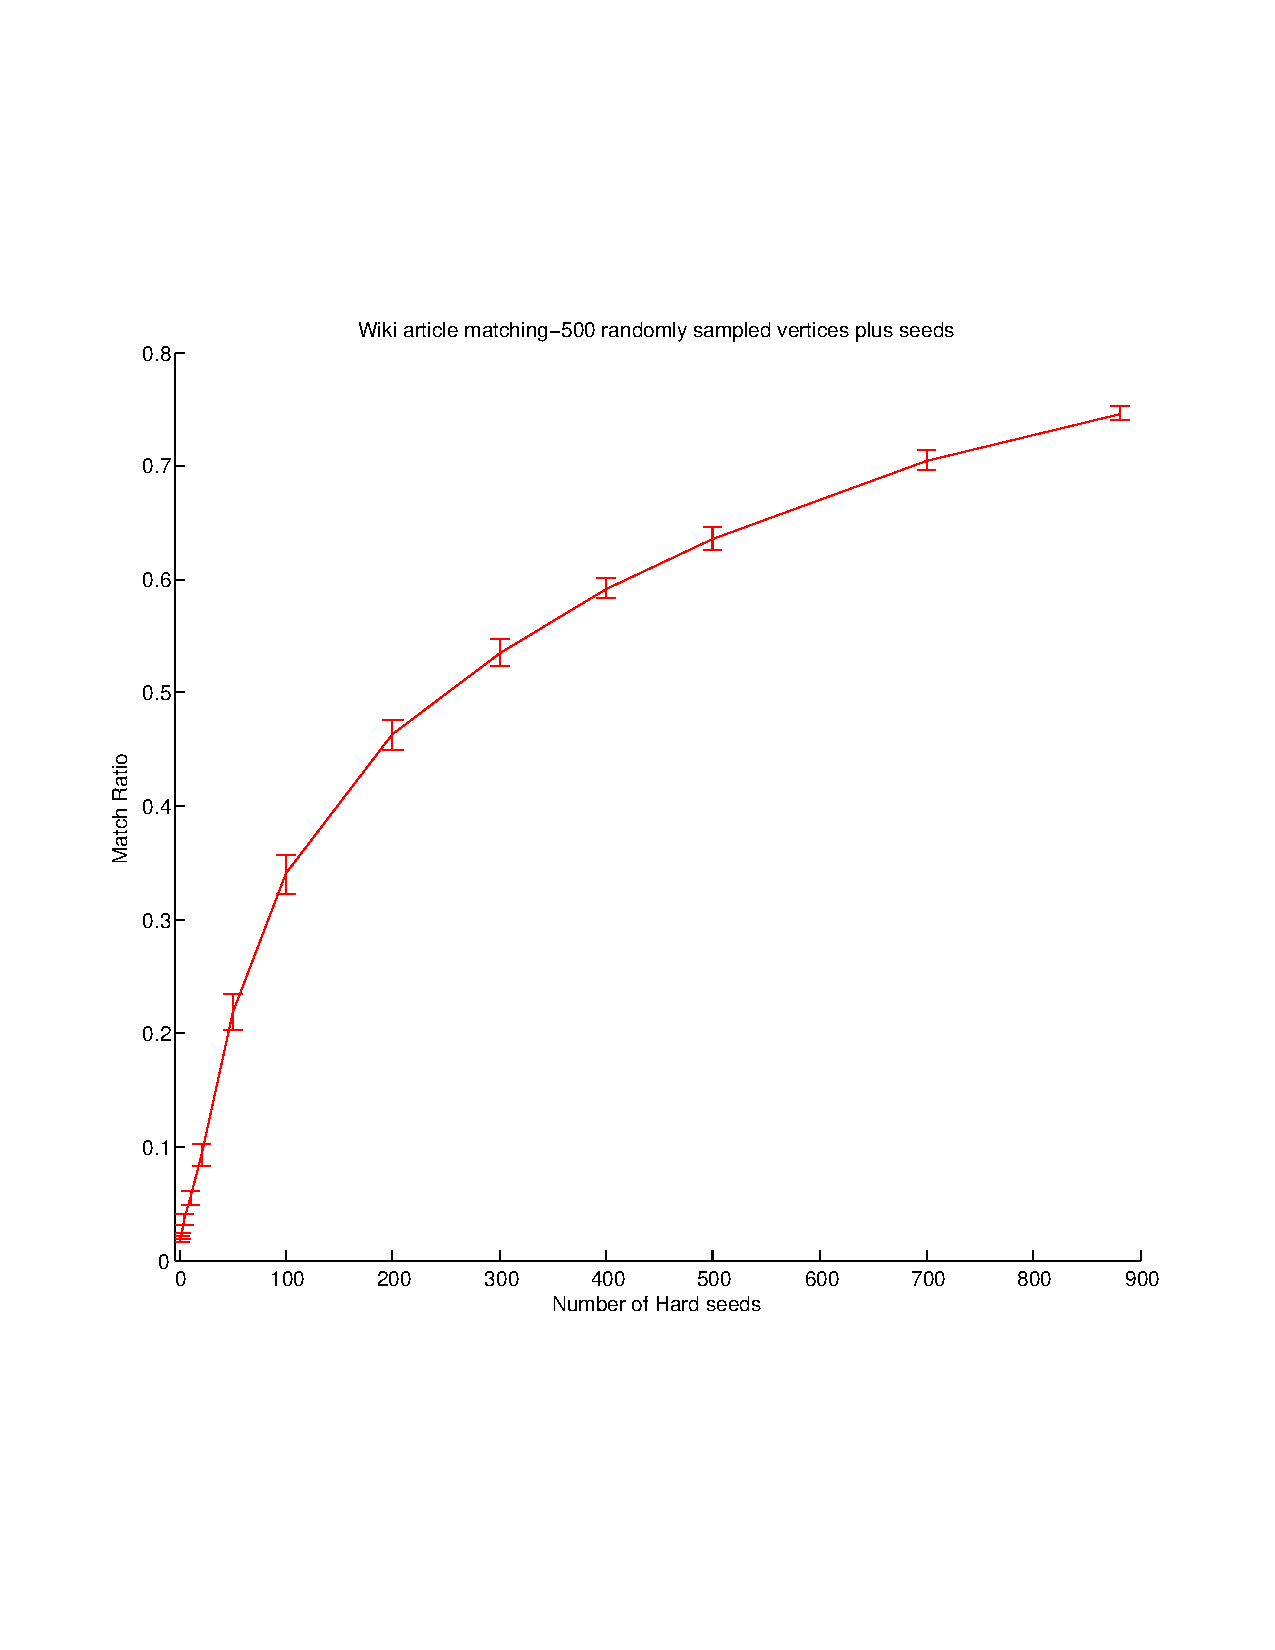
\includegraphics[scale=0.8]{wiki}
\caption{Matching English and French subgraphs \label{Wiki-fig-1}  }
\end{figure}

This example is the most computationally expensive of our examples. Figure \ref{Wiki-fig-2} shows the running time vs number of vertices to be matched.

\begin{figure}
\centering
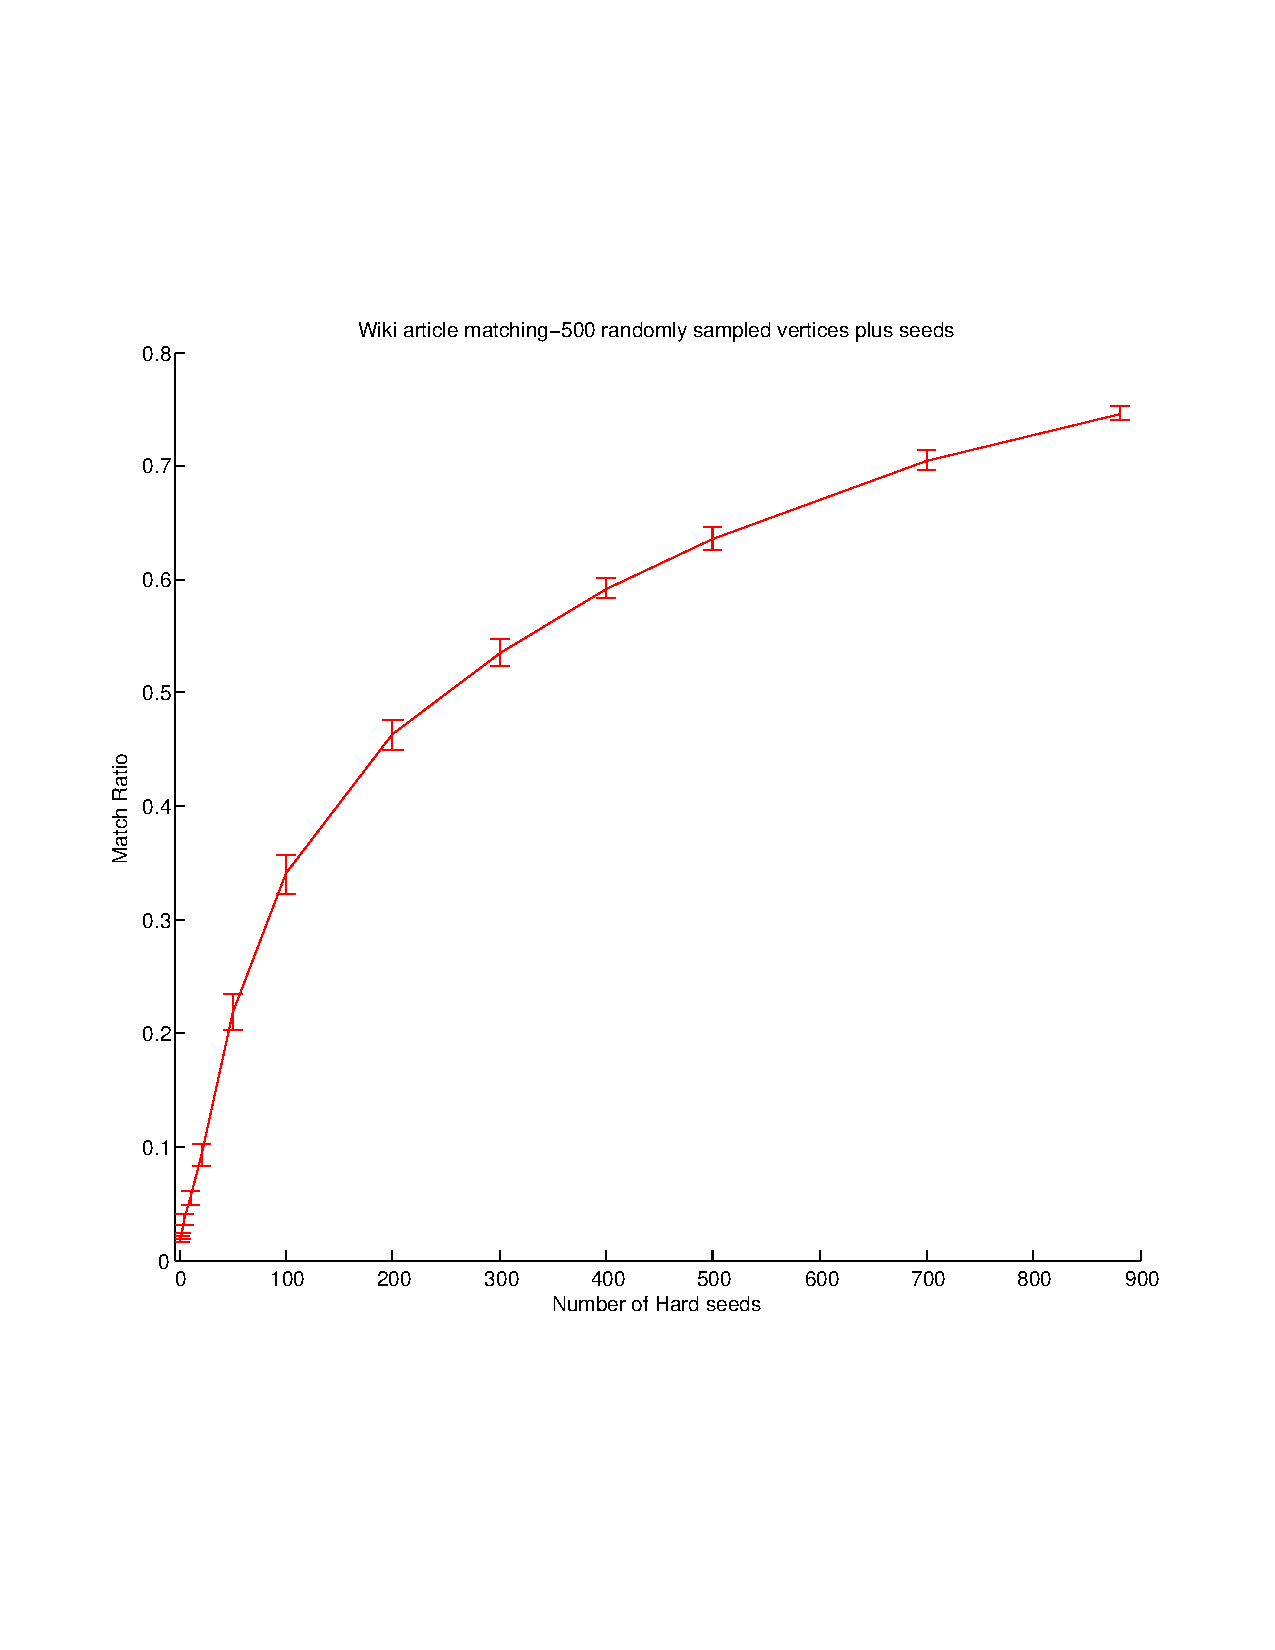
\includegraphics[scale=0.8]{wiki}
\caption{Matching English and French subgraphs \label{Wiki-fig-1}  }
\end{figure}

\section{Caenorhabditis elegans brain example \label{celegans}}
C. elegans is a worm that is a model organism that has been extensively studied. Its  particular usefulness comes from its nervous system, consisting of 302 neurons whose connectome have been  mapped \cite{}. There are two types  of  connections between neurons: chemical( chemical synapses) and electrical(junction potentials ). 

INSERT REASON for 279 vertex graph instead of 302.

The objective of the experiment is to match the chemical graph $G_1$ to  the electrical one $G_2$ .  The adjacency matrices for both graphs are sparse.  Both $G_1$ and $G_2$ are weighted graphs, i.e each edge has a nonzero real number attribute, so for sake of uniformity with the other examples, the adjacency matrices are binarized and symmetrized.  For each number of hard seeds, $m \in\{0,1,5,10,20,50,75,100,150,200\}$,  there are different number of vertices to be matched $n=k-m$. Since the expected number of matches is always 1, the match ratio for random chance $\frac{1}{n}$ is different for each different number of hard seeds. Note the increasing random chance curve in Fig. \ref{worm-fig}.
\begin{figure}
\centering
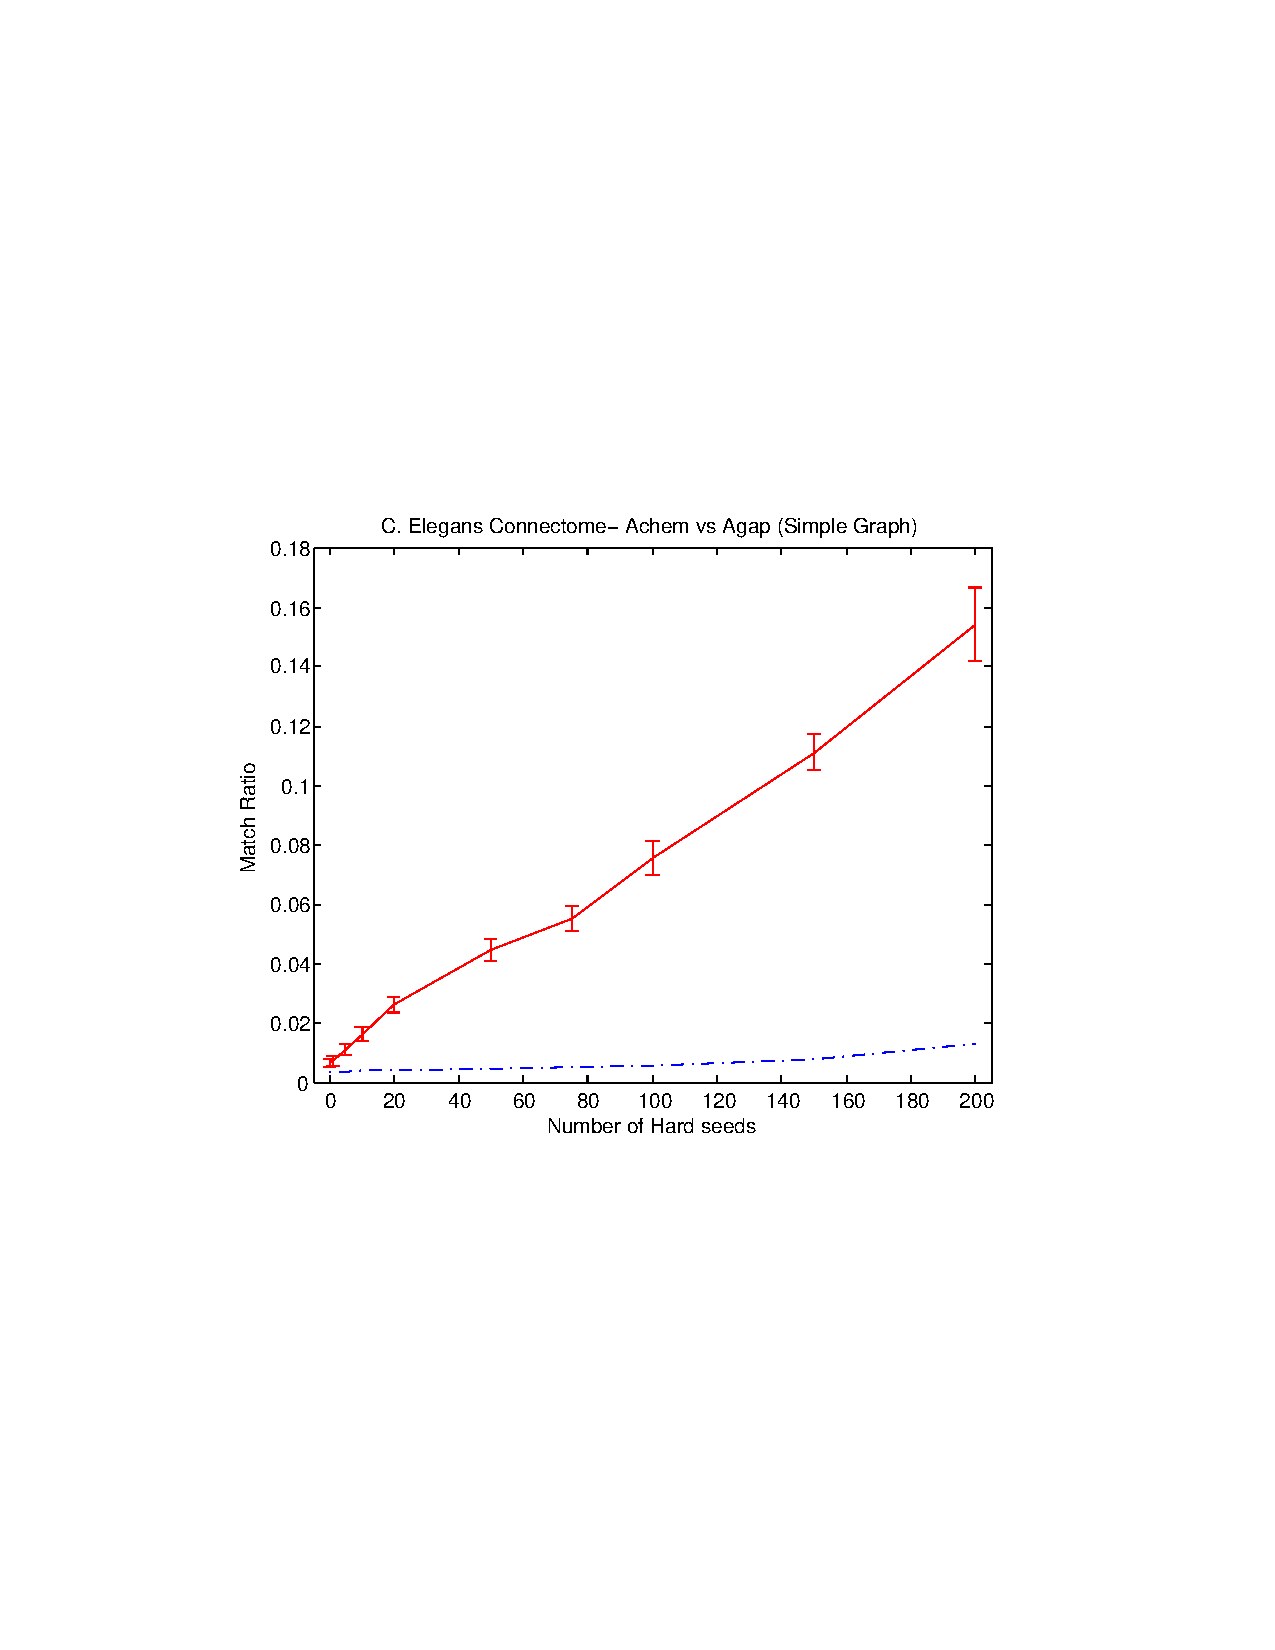
\includegraphics[scale=.8]{worm}
\caption{Matching of Chemical and Electrical connectivity graphs of C. elegans nervous system \label{worm-fig}  }
\end{figure}

Although the match ratio is generally low which should be expected due to the difficulty of the problem, increasing number of hard seeds results in a consistent increase in match ratio.

\section{Enron example \label{enron}}
Enron email corpus consists of mails between $k=184$ employees in Enron. Publicly available emails are used to compute a time-series of graphs $\{G_t, t=1,\ldots,T\}$ between $k$ vertices. The inference task is to find anomalies(schemers scheming to commit fraud) in this communication graph.    
Previous work \cite{} indicates suspicious behaviour takes place at time stamps $t=(130,131,132)$. .  Graphs with consecutive  timesteps at $t=(130,131,132)$ are matched one pair at a time using modified-FAQ. The match ratio for each pair is plotted in \ref{enron-fig}.

\begin{figure}
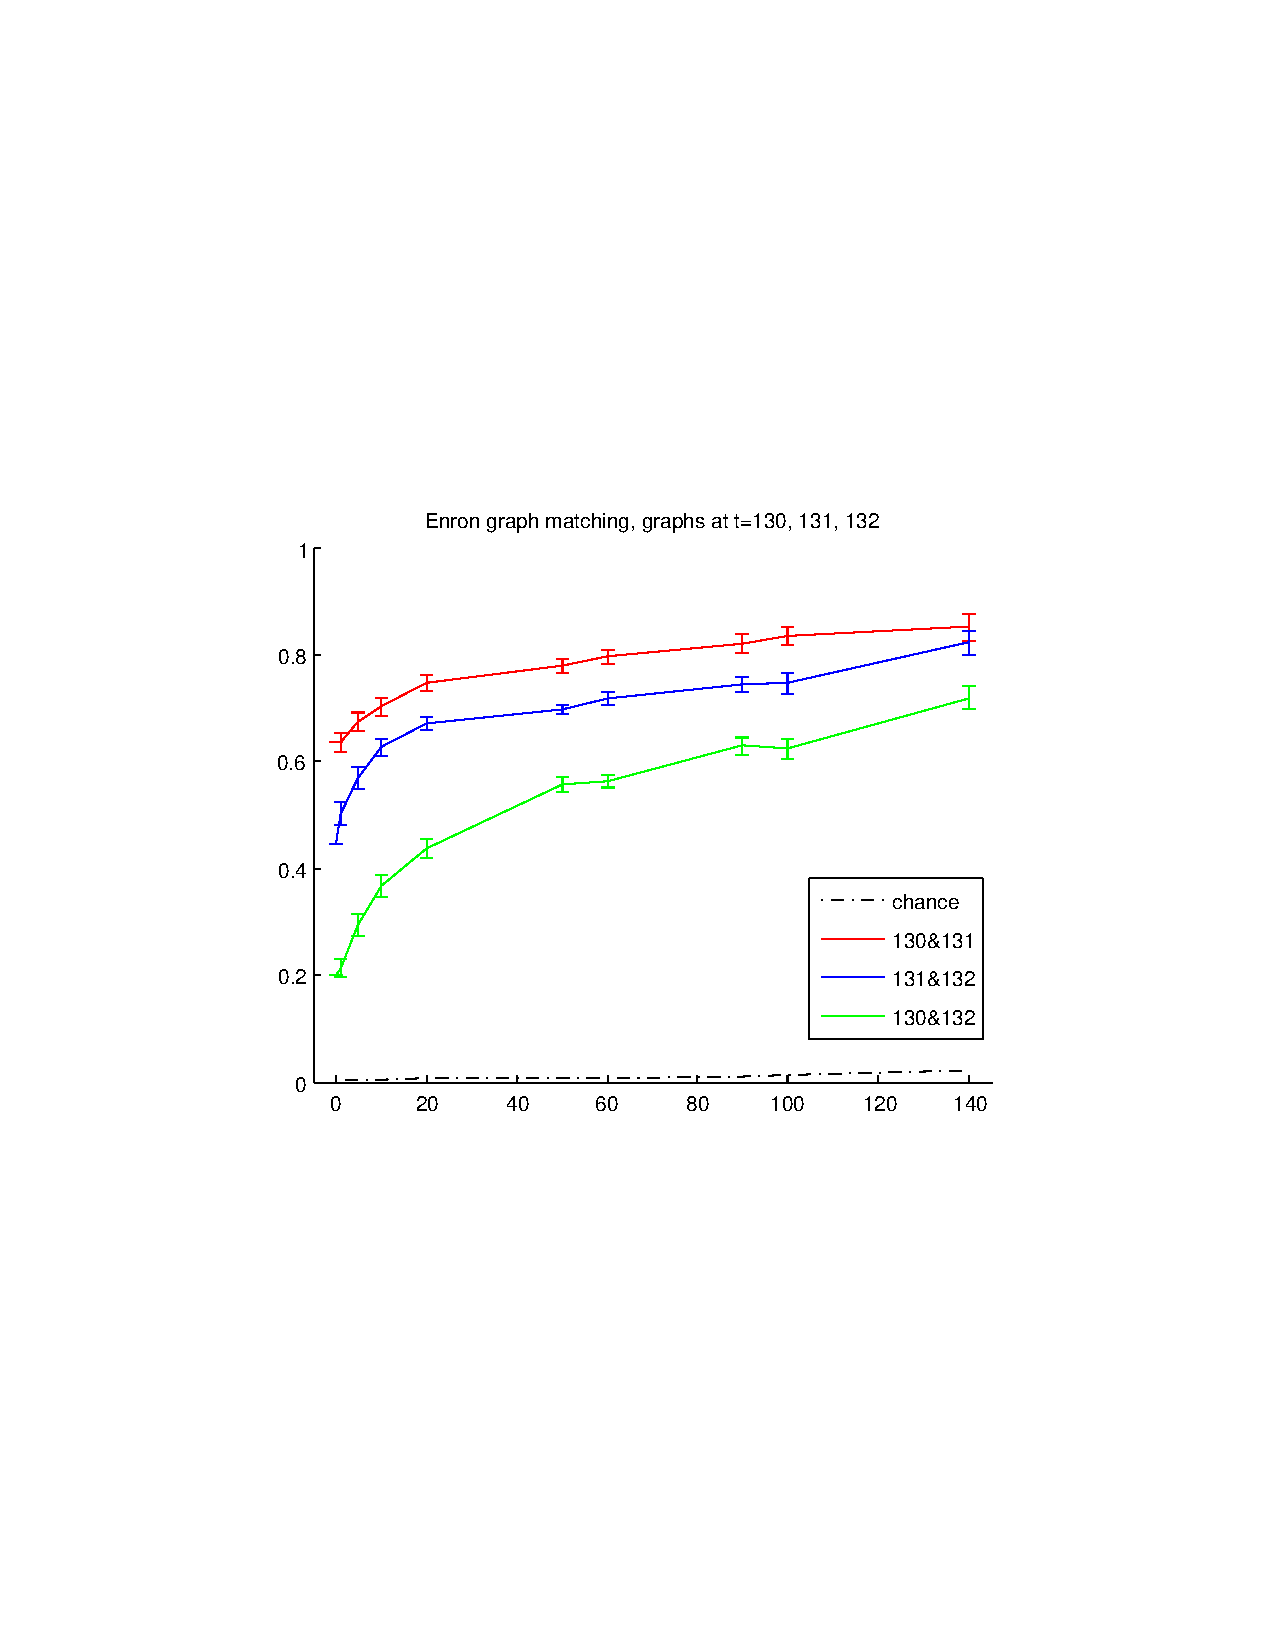
\includegraphics[scale=0.8]{enron}
\caption{Matching of Enron communication graph at timestamps: 130,131,132 \label{enron-fig}  }
\end{figure}

The results are consistent with previous work \cite{}, the average match ratio is much higher between the graphs at $t=130$ and $t=131$ compared to matching between $t=131$ and $t=132$  and between $t=130$ and $t=132$.  The anomalous event in the graph time-series takes place at  $t=132$ according to \cite{}, which makes the graph matching more difficult compared to matching graphs at other times. 

Note that the Two-Class experiment is an appropriate model for this problem.  The list of anomalous  vertices (scheming fraudsters) , as detected by \cite{} , are 
$ \{v\in V : \gamma(v)=1\} =  \{
    2 ,  3 ,  4,   5,   7 , 10,  11,  17 , 18 , 19  ,22 , 28 , 31 , 33,  40,  41 , 44  ,46,  47 ,
  48,  50 , 52,  54 , 55,  57  ,59,  60  ,63  ,64 , 65,\linebreak 
 ,71 , 76  ,77 , 79,  80 , 83 , 84,  85, 
  86 , 87  ,89 , 90  ,94 , 97 , 98 ,102 ,103 ,107, 108, 113, 115 ,117, 119 ,120, 126 , \linebreak
127, 128 ,
130 ,133 ,134, 137, 138 ,140, 141, 144 ,146 ,147, 148 ,149 ,150, 155 ,157, 158, 160, 164, 165, \linebreak
 167 ,174, 176, 177, 180 ,183 \}$





\begin{thebibliography}{9}

\bibitem{sixteen}
   H.A. Almohamad and S.O. Duffuaa,
   A linear programming approach for the weighted
   graph matching problem,
   \emph{IEEE Transactions on Pattern Analysis and Machine Intelligence}
   {\bf 15} (1993) pp 522--525.

\bibitem{Thirty}
   D. Conte, P. Foggia, C. Sansone, and M. Vento,
   Thirty years of graph matching in pattern recognition,
   \emph{International Journal of Pattern Recognition and
   Artificial Intelligence} {\bf 18} (2004) pp 265--298.

\bibitem{VogCon}
    J.T. Vogelstein, J.M. Conroy, L.J. Podrazik,
    S.G. Kratzer, E.T. Harley, D.E. Fishkind,
    R.J. Vogelstein, and C.E. Priebe,
    Brain graph matching via fast approximate quadratic programming,
    submitted. Available at arxiv.org/pdf/1112.5507



\end{thebibliography}

\end{document}
